\documentclass[14pt]{extbook}
\usepackage{multicol, enumerate, enumitem, hyperref, color, soul, setspace, parskip, fancyhdr} %General Packages
\usepackage{amssymb, amsthm, amsmath, bbm, latexsym, units, mathtools} %Math Packages
\everymath{\displaystyle} %All math in Display Style
% Packages with additional options
\usepackage[headsep=0.5cm,headheight=12pt, left=1 in,right= 1 in,top= 1 in,bottom= 1 in]{geometry}
\usepackage[usenames,dvipsnames]{xcolor}
\usepackage{dashrule}  % Package to use the command below to create lines between items
\newcommand{\litem}[1]{\item#1\hspace*{-1cm}\rule{\textwidth}{0.4pt}}
\pagestyle{fancy}
\lhead{Progress Quiz 1}
\chead{}
\rhead{Version C}
\lfoot{3114-1073}
\cfoot{}
\rfoot{Fall 2020}
\begin{document}

\begin{enumerate}
\litem{
Solve the equation below. Then, choose the interval that contains the solution.\[ -17(4x + 12) = -3(2x + 15) \]\begin{enumerate}[label=\Alph*.]
\item \( x \in [-4.23, -3.85] \)
\item \( x \in [-3.04, -2.19] \)
\item \( x \in [-3.79, -3.01] \)
\item \( x \in [3.92, 4.15] \)
\item \( \text{There are no real solutions.} \)

\end{enumerate} }
\litem{
Solve the linear equation below. Then, choose the interval that contains the solution.\[ \frac{5x -8}{8} - \frac{-8x -9}{3} = \frac{9x -7}{5} \]\begin{enumerate}[label=\Alph*.]
\item \( x \in [-6, -5.2] \)
\item \( x \in [-1.9, -0.1] \)
\item \( x \in [-3.5, -1.1] \)
\item \( x \in [0.7, 2.1] \)
\item \( \text{There are no real solutions.} \)

\end{enumerate} }
\litem{
Write the equation of the line in the graph below in Standard form $Ax+By=C$. Then, choose the intervals that contain $A, B, \text{ and } C$.
\begin{center}
    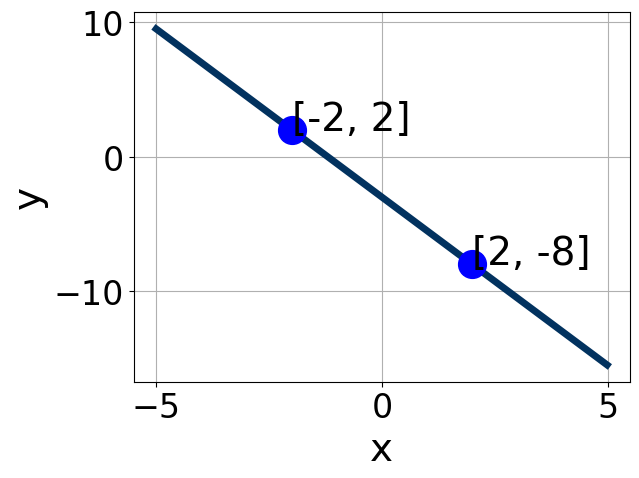
\includegraphics[width=0.5\textwidth]{../Figures/linearGraphToStandardC.png}
\end{center}
\begin{enumerate}[label=\Alph*.]
\item \( A \in [-3, -1], \hspace{3mm} B \in [2.7, 6.6], \text{ and } \hspace{3mm} C \in [6, 9] \)
\item \( A \in [1, 6], \hspace{3mm} B \in [2.7, 6.6], \text{ and } \hspace{3mm} C \in [6, 9] \)
\item \( A \in [1, 6], \hspace{3mm} B \in [-4.7, -3.5], \text{ and } \hspace{3mm} C \in [-9, -7] \)
\item \( A \in [-2.75, 0.25], \hspace{3mm} B \in [-1.8, -0.1], \text{ and } \hspace{3mm} C \in [-6, -1] \)
\item \( A \in [-2.75, 0.25], \hspace{3mm} B \in [0.6, 2.7], \text{ and } \hspace{3mm} C \in [0, 6] \)

\end{enumerate} }
\litem{
Find the equation of the line described below. Write the linear equation as $ y=mx+b $ and choose the intervals that contain $m$ and $b$.\[ \text{Parallel to } 5 x - 7 y = 13 \text{ and passing through the point } (10, 7). \]\begin{enumerate}[label=\Alph*.]
\item \( m \in [-1.02, -0.22] \hspace*{3mm} b \in [13.78, 14.59] \)
\item \( m \in [0.65, 1.15] \hspace*{3mm} b \in [0.08, 0.45] \)
\item \( m \in [0.65, 1.15] \hspace*{3mm} b \in [-0.5, 0.1] \)
\item \( m \in [1.2, 1.88] \hspace*{3mm} b \in [-0.5, 0.1] \)
\item \( m \in [0.65, 1.15] \hspace*{3mm} b \in [-3.23, -2.58] \)

\end{enumerate} }
\litem{
First, find the equation of the line containing the two points below. Then, write the equation as $ y=mx+b $ and choose the intervals that contain $m$ and $b$.\[ (5, 4) \text{ and } (-9, 2) \]\begin{enumerate}[label=\Alph*.]
\item \( m \in [-0.04, 1.1] \hspace*{3mm} b \in [2.63, 4.19] \)
\item \( m \in [-0.34, 0.08] \hspace*{3mm} b \in [0.26, 0.88] \)
\item \( m \in [-0.04, 1.1] \hspace*{3mm} b \in [10.67, 11.29] \)
\item \( m \in [-0.04, 1.1] \hspace*{3mm} b \in [-3.74, -3.24] \)
\item \( m \in [-0.04, 1.1] \hspace*{3mm} b \in [-1.02, -0.74] \)

\end{enumerate} }
\litem{
Solve the equation below. Then, choose the interval that contains the solution.\[ -17(4x -14) = -13(-5x + 11) \]\begin{enumerate}[label=\Alph*.]
\item \( x \in [-1.03, -0.61] \)
\item \( x \in [31.42, 32.35] \)
\item \( x \in [0.46, 0.77] \)
\item \( x \in [2.43, 3.1] \)
\item \( \text{There are no real solutions.} \)

\end{enumerate} }
\litem{
First, find the equation of the line containing the two points below. Then, write the equation as $ y=mx+b $ and choose the intervals that contain $m$ and $b$.\[ (5, 11) \text{ and } (-9, -6) \]\begin{enumerate}[label=\Alph*.]
\item \( m \in [-0.2, 3.4] \hspace*{3mm} b \in [5.3, 7.4] \)
\item \( m \in [-0.2, 3.4] \hspace*{3mm} b \in [3.6, 5.4] \)
\item \( m \in [-0.2, 3.4] \hspace*{3mm} b \in [-6.6, -4.3] \)
\item \( m \in [-0.2, 3.4] \hspace*{3mm} b \in [-1.4, 3.9] \)
\item \( m \in [-3.6, 0] \hspace*{3mm} b \in [-17.2, -15] \)

\end{enumerate} }
\litem{
Write the equation of the line in the graph below in Standard form $Ax+By=C$. Then, choose the intervals that contain $A, B, \text{ and } C$.
\begin{center}
    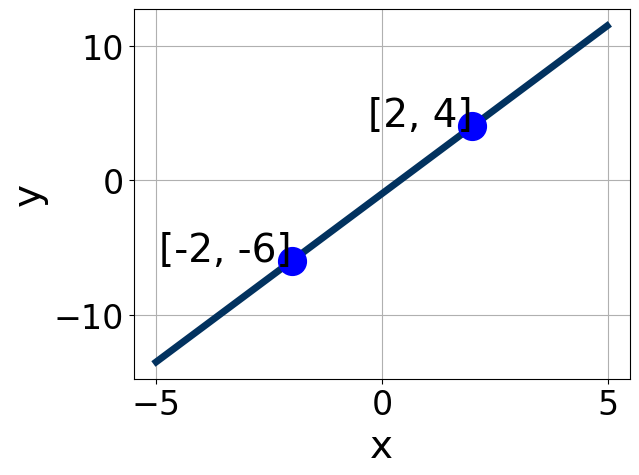
\includegraphics[width=0.5\textwidth]{../Figures/linearGraphToStandardCopyC.png}
\end{center}
\begin{enumerate}[label=\Alph*.]
\item \( A \in [-7, -3], \hspace{3mm} B \in [1.62, 4.26], \text{ and } \hspace{3mm} C \in [-7.2, -4] \)
\item \( A \in [-3.33, -0.33], \hspace{3mm} B \in [0.99, 1.45], \text{ and } \hspace{3mm} C \in [-4.9, -1.3] \)
\item \( A \in [-3.33, -0.33], \hspace{3mm} B \in [-1.68, -0.17], \text{ and } \hspace{3mm} C \in [1.5, 2.9] \)
\item \( A \in [0, 8], \hspace{3mm} B \in [-4.23, -2.86], \text{ and } \hspace{3mm} C \in [4.3, 8.9] \)
\item \( A \in [0, 8], \hspace{3mm} B \in [1.62, 4.26], \text{ and } \hspace{3mm} C \in [-7.2, -4] \)

\end{enumerate} }
\litem{
Solve the linear equation below. Then, choose the interval that contains the solution.\[ \frac{3x + 8}{2} - \frac{7x -5}{4} = \frac{-8x -7}{5} \]\begin{enumerate}[label=\Alph*.]
\item \( x \in [-5.2, -3.9] \)
\item \( x \in [-2.1, -1.2] \)
\item \( x \in [-14.9, -13.5] \)
\item \( x \in [-4.5, -3] \)
\item \( \text{There are no real solutions.} \)

\end{enumerate} }
\litem{
Find the equation of the line described below. Write the linear equation as $ y=mx+b $ and choose the intervals that contain $m$ and $b$.\[ \text{Parallel to } 9 x + 8 y = 10 \text{ and passing through the point } (9, 7). \]\begin{enumerate}[label=\Alph*.]
\item \( m \in [1.07, 1.26] \hspace*{3mm} b \in [-4.2, -2.7] \)
\item \( m \in [-1.4, -1.12] \hspace*{3mm} b \in [-2.9, -1.3] \)
\item \( m \in [-1.4, -1.12] \hspace*{3mm} b \in [16.6, 18.6] \)
\item \( m \in [-0.95, -0.85] \hspace*{3mm} b \in [16.6, 18.6] \)
\item \( m \in [-1.4, -1.12] \hspace*{3mm} b \in [-19.6, -16.1] \)

\end{enumerate} }
\end{enumerate}

\end{document}